\section{Methodology}
\label{sec:methodology}

\begin{figure}[t]
  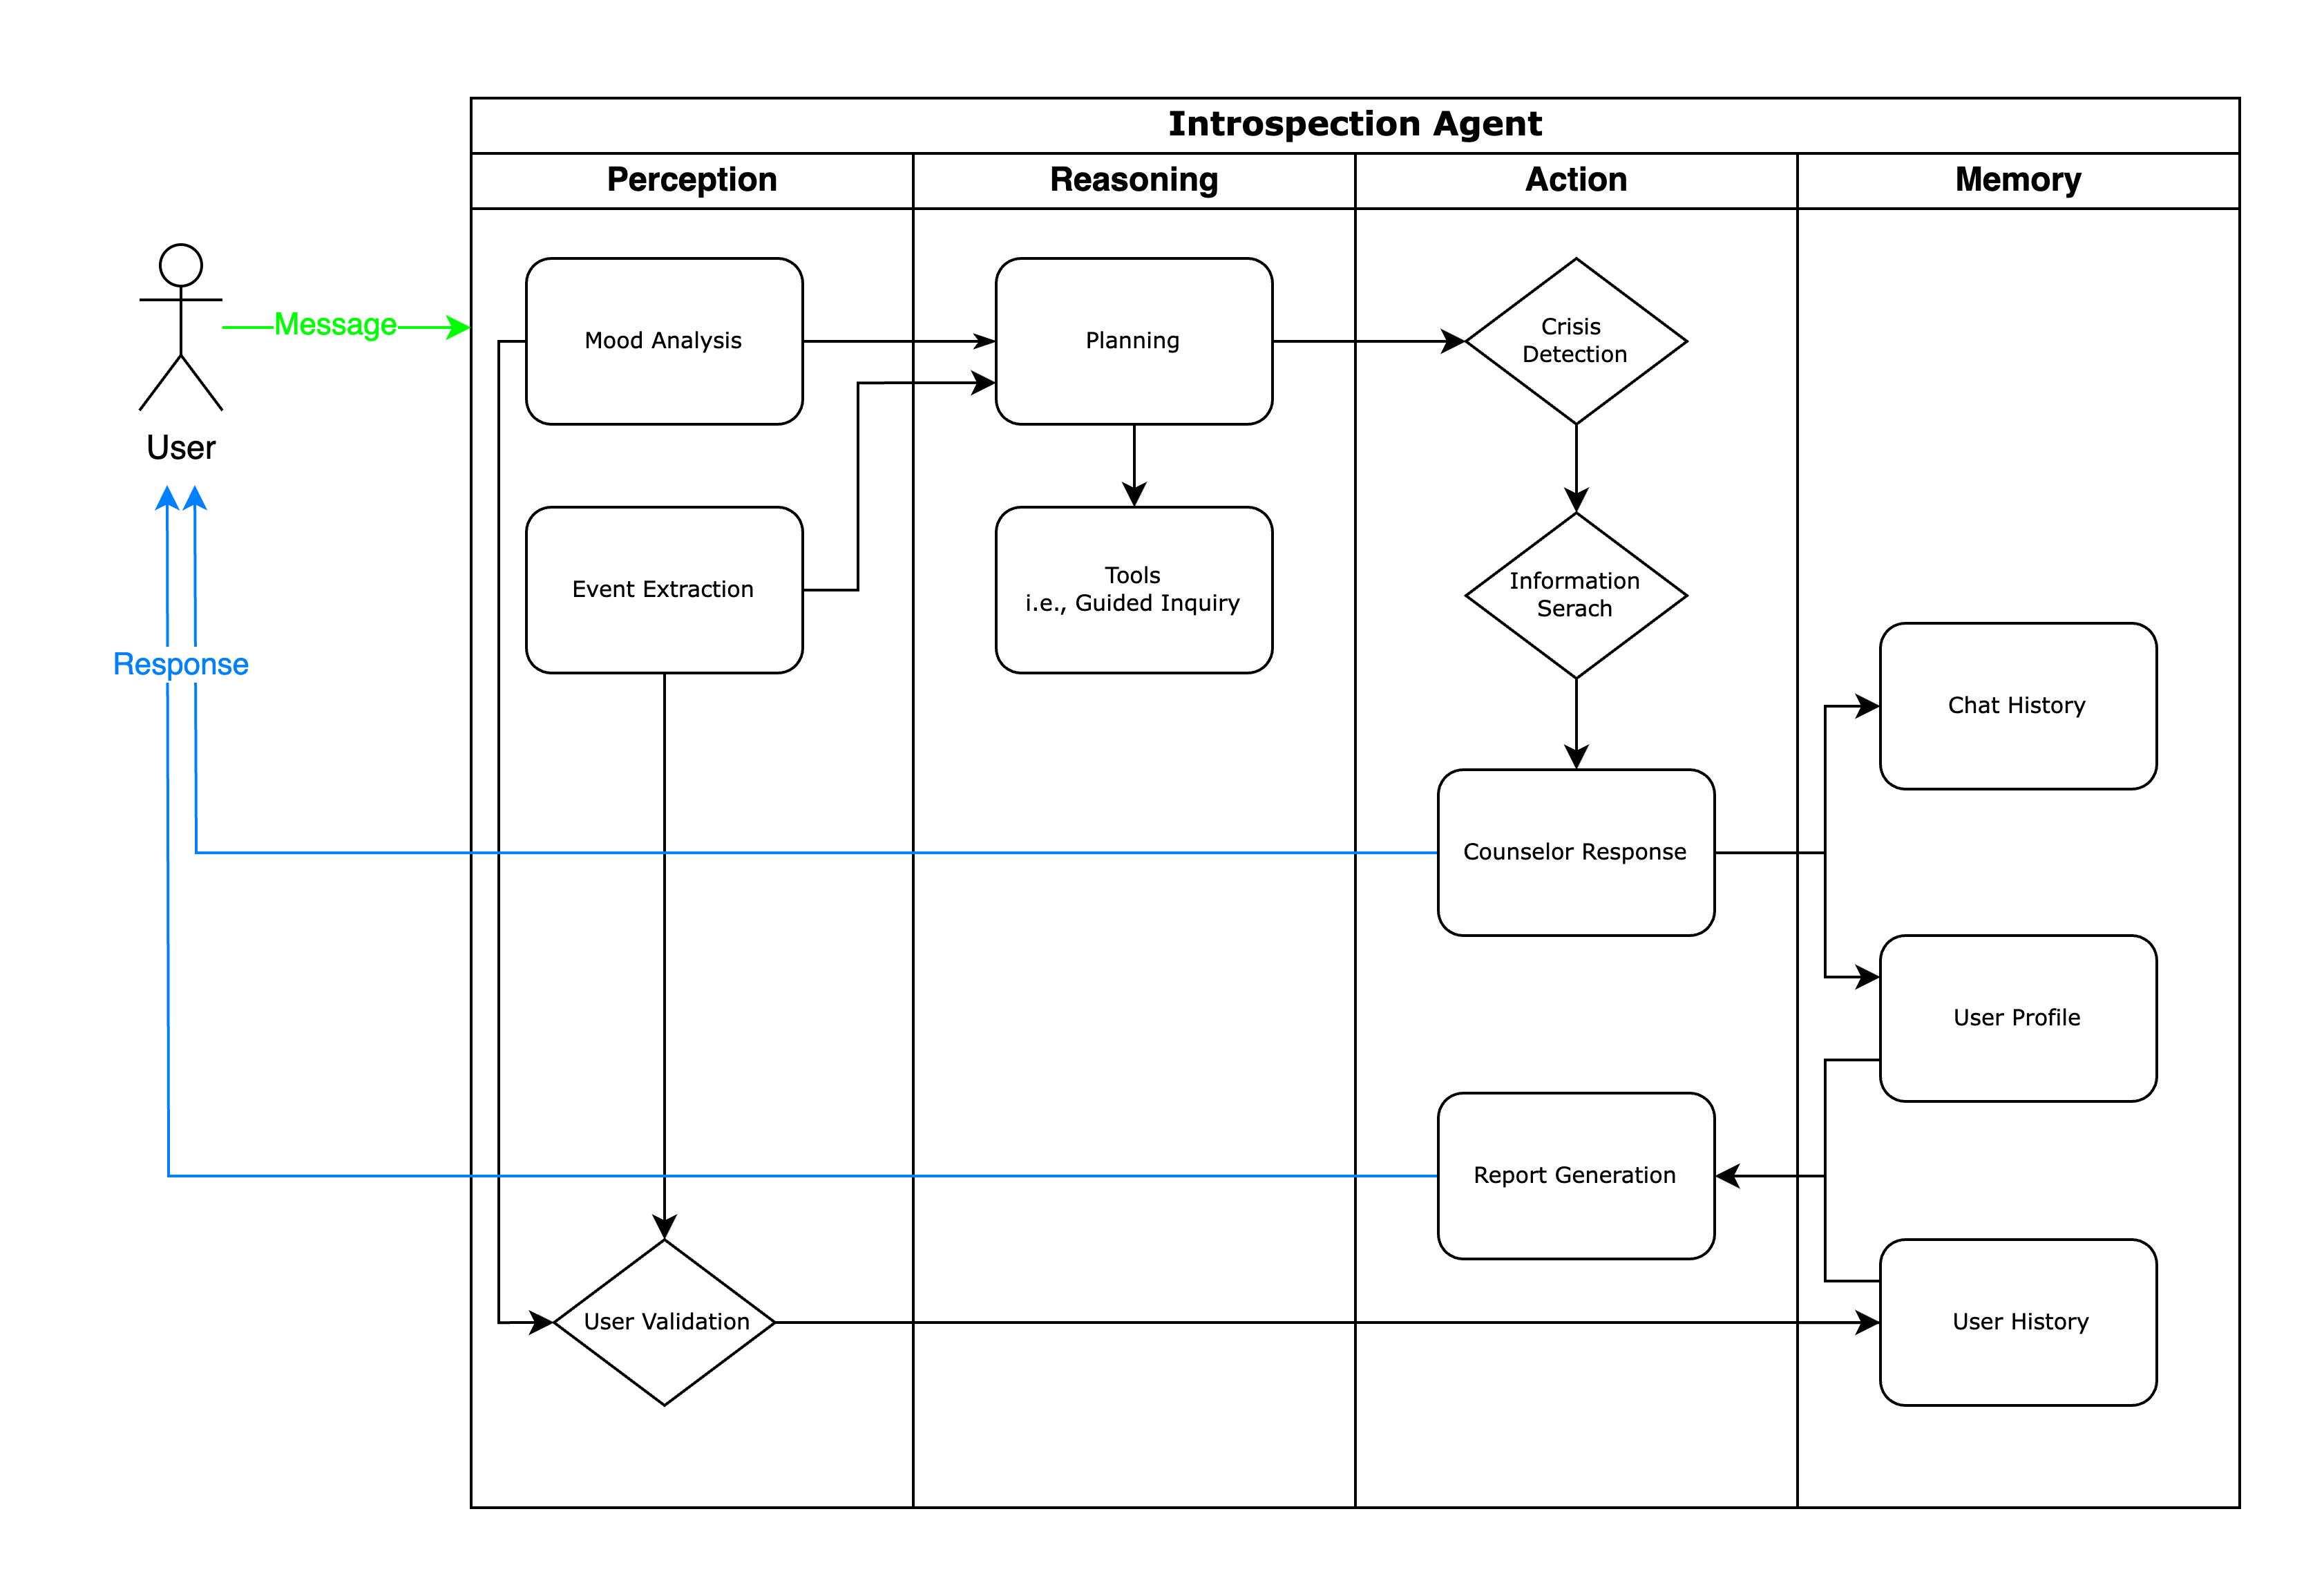
\includegraphics[width=\columnwidth]{figs/introspection-agent.png}
  \caption{An overview of introspection agent.}
  \label{fig:introspection-agent}
\end{figure}

In this section, we first provide an overview of how the Introspection Agent operates, followed by a detailed discussion of its main components.

As illustrated in Figure~\ref{fig:introspection-agent}, the agent is organized into four key modules: \textbf{Perception}, \textbf{Reasoning}, \textbf{Action}, and \textbf{Memory}. Upon receiving user input, the system initially performs \textit{Mood Analysis} and \textit{Event Extraction} to interpret the user's emotional state and contextual information. The \textbf{Reasoning} module then engages in \textit{Planning} and leverages tools such as \textit{Guided Inquiry} to process the user's request. If a potential crisis is detected (\textit{Crisis Detection}), the system immediately enters a crisis intervention phase and provides a psychological help hotline. If a search intent is identified, the system conducts an \textit{Information Search} before generating a \textit{Counselor Response}. 

Throughout this process, all interactions are systematically logged in the \textit{Chat History}, \textit{User Profile}, and \textit{User History}, enabling continuous learning and personalized user experiences.

\subsection{Perception}

\subsubsection{Mood}

The mood analysis feature represents a sophisticated integration of large language model (LLM) capabilities with clinical psychology principles, specifically designed to provide continuous, contextually-aware emotional evaluation.

\paragraph{Data Structure}

The analytical foundation leverages meticulously engineered prompts that instruct the LLM to function as an emotion analysis expert, ensuring consistent and clinically-relevant outputs. This prompt engineering approach directs the model to analyze conversational data and return a structured JSON schema encompassing four fundamental dimensions that align with established psychological frameworks, particularly Cognitive Behavioral Therapy (CBT) principles.

\begin{itemize}
\item \textbf{Mood Intensity:} A normalized scalar value ranging from 0 to 10, providing a quantitative measure of emotional arousal. This continuous scale enables nuanced tracking of emotional fluctuations and facilitates longitudinal analysis of affective patterns.

\item \textbf{Mood Category:} A discrete emotional classification drawn from a comprehensive taxonomy of psychological states (e.g., Sad,'' Anxious,'' ``Excited''). This categorical approach aligns with established psychological frameworks while maintaining sufficient granularity for clinical relevance.

\item \textbf{Thinking:} A verbatim quote or paraphrased representation of the user's potential inner monologue or cognitive appraisals (e.g., ``I am a failure''). This dimension serves as a critical component for identifying cognitive distortions, a fundamental concept in Cognitive Behavioral Therapy (CBT), enabling therapeutic interventions targeting maladaptive thought patterns.

\item \textbf{Scene:} The contextual trigger or situational antecedent associated with the emotional response (e.g., ``Seeing a friend's post on social media''). This contextual grounding facilitates the identification of environmental triggers and supports the development of situation-specific coping strategies.
\end{itemize}

This multi-faceted analytical framework transcends traditional sentiment analysis by providing a comprehensive psychological profile that captures not merely the valence and arousal of emotions, but also their cognitive and contextual underpinnings.

\paragraph{Technical Implementation Architecture}

\textbf{MoodService }\\
The system implements a dedicated LLM-based analytical service, designated as the MoodService, which operates through a discrete LLM instance (specifically, Qwen3-32B) to ensure computational independence from primary conversational functions. This service is governed by meticulously engineered prompts, which constrains model outputs to conform to predefined analytical specifications while maintaining focus on comprehensive psychological evaluation. In addition, the architectural segregation  ensures that intensive mood analysis computations do not compromise real-time conversational responsiveness, thereby preserving user experience integrity.

\textbf{Contextual Batch Processing}\\
The system employs a sliding window methodology for contextual message processing, systematically extracting and analyzing the seven most recent user messages subsequent to each conversational interaction. This temporal windowing approach facilitates the incorporation of conversational context essential for accurate emotional state detection while enabling the identification of emotional progression patterns rather than discrete affective snapshots. 

\textbf{Feedback Integration}

To optimize user experience and prevent cognitive overload, the system implements an intelligent refresh algorithm for mood data updates that operates under dual criteria: when mood intensity exceeds 0.8 on the normalized scale, indicating emotionally significant states, and when the detected mood category differs from the previous assessment, preventing redundant notifications. This approach ensures users receive alerts only for meaningful emotional transitions, reducing notification fatigue while maintaining clinical relevance and therapeutic value.

Upon navigation to the mood analysis interface, the system presents automatically generated emotional assessments in a structured, visually accessible format with mood intensity, category, cognitive content, and situational context displayed in an initially read-only state, allowing users to inspect assessments without inadvertent modification. The system incorporates feedback mechanisms through editing functionality that enable users to correct misidentified emotional states or contextual elements. All user interactions include real-time UI feedback through toast notifications and visual state indicators, ensuring transparency and maintaining engagement throughout the assessment process.

\textbf{Data Management}

The system's backend architecture supports comprehensive data management through structured data transmission using RESTful API endpoints with standardized JSON schemas, ensuring data integrity and interoperability across system components. Each mood record incorporates session identifiers and temporal metadata, enabling accurate longitudinal tracking and user-specific analysis patterns essential for monitoring.


\subsubsection{Event}

\begin{figure}[h]
    \centering
    \includegraphics[width=0.8\columnwidth]{figs/LLM4IE.jpg}
    \caption{Overview of Large Language Model-based Information Extraction Frameworks~\cite{xu2023large}.}
    \label{fig:LLM4IE}
\end{figure}

\paragraph{Event-Driven Reflection}
A cornerstone of our methodology is the principle of event-driven reflection. As illustrated in Figure~\ref{fig:LLM4IE}, large language models (LLMs) have been extensively explored for generative information extraction (IE), encompassing various IE techniques, specialized frameworks for single subtasks, and universal frameworks capable of addressing multiple subtasks simultaneously. We posit that significant psychological insight is often anchored to specific life events. Rather than merely providing conversational support, our system is designed to function as a non-judgmental mirror, empowering users to identify, structure, and reflect upon these pivotal moments. As outlined in our initial proposal, the core value of this mechanism lies not in AI-driven judgment, but in providing users with a structured and objective record of their own experiences. This approach transforms raw conversational data into a curated timeline of personal growth, facilitating self-discovery and fostering a deeper understanding of one's own emotional and cognitive patterns. The entire event mechanism is designed to be user-centric, granting users full agency to accept, modify, or discard the AI's interpretations, thereby ensuring the final record is a faithful representation of their personal narrative.

\begin{figure}[!b]
    \centering
    \includegraphics[width=0.6\columnwidth]{figs/event-extraction-pipeline.jpg}
    \caption{Overview of Event Extraction Architecture}
    \label{fig:event-pipeline}
\end{figure}

\paragraph{Asynchronous Event Extraction}

To technically realize the principle of event-driven reflection, we implement an asynchronous Event Extraction (EE) pipeline, as shown in Figure~\ref{fig:event-pipeline}. Formulated as a generative information extraction task\cite{xu2023large}, its primary objective is to distill unstructured user dialogues into structured representations of psychologically significant events. This pipeline operates in the background, decoupled from the main chat interface, to ensure a seamless user experience without interrupting the conversational flow. It is triggered automatically based on conversational cues, specifically after every three turns of dialogue. Upon activation, the service retrieves the recent conversation history and processes it to identify and extract key events.

The integrity and utility of our system hinge on the quality of this extracted data. To this end, we have implemented several key mechanisms to ensure high-fidelity, structured output:

\begin{itemize}
    \item \textbf{Standardized Event Schema.} We define a rigid JSON schema for event representation, encapsulating essential fields such as \texttt{primaryType}, \texttt{subType}, \texttt{title}, and \texttt{content}. This schema categorizes events across multiple psychological dimensions (e.g., emotional, relational, cognitive), providing a consistent and machine-readable format for subsequent analysis. This functionality is enabled by the constrained decoding capabilities provided by inference engines such as vLLM and SGLang, which allow us to enforce the required structure by specifying the \texttt{response\_format=\{"type": "json\_object"\}} parameter in the LLM API call. It directly addresses the common challenge of misalignment between the LLM's natural language output and the required structured form \cite{xu2023large}.

    \item \textbf{Dedicated Processing Service.} The EE task is managed by a dedicated microservice, the \textit{EventService}, which utilizes a separate LLM instance (i.e., DeepSeek-V3) from the primary conversational agent. This architectural choice serves a dual purpose: it allows for task-specific model optimization and prevents potential API rate-limiting issues that could arise from overloading a single model endpoint, thereby safeguarding the responsiveness of the main dialogue.

    \item \textbf{User-in-the-Loop Validation.} Recognizing the potential for LLM-induced hallucinations, we incorporate a user-in-the-loop validation mechanism. Extracted events are presented to the user as editable cards within the application's interface. Users are granted full agency to review, confirm, modify, or delete any event. This process not only acts as a crucial safeguard for data fidelity but also enhances user trust and engagement by maintaining transparency and user control over their personal data. The system only commits events to the long-term storage---a lightweight, file-based system organized by session ID---upon explicit user confirmation.
\end{itemize} 

\subsection{Reasoning}

\subsubsection{Planning}

The Planning module is responsible for analyzing the user's intent and dynamically generating a dialogue strategy to guide the conversation. Upon receiving new user input, the system retrieves the current plan from persistent storage or initializes a new plan if none exists. The plan is structured as a JSON object containing fields such as \texttt{user\_intent}, \texttt{current\_state}, \texttt{steps}, \texttt{context}, and \texttt{inquiry\_status}. 

A dedicated prompt is used to instruct the LLM to update the plan based on the latest user message and conversation history. The LLM analyzes the user's needs, updates the dialogue steps, and refines the inquiry strategy. Each step in the plan is tracked with a status (e.g., ``pending'', ``in progress'', ``completed''), allowing for iterative and adaptive planning as the conversation evolves. The updated plan is then stored and used to inform subsequent system actions, ensuring that responses are purposeful, context-aware, and aligned with the user's goals.

This modular planning approach enables the agent to maintain coherence across multi-turn dialogues, adapt to new information, and provide structured guidance throughout the counseling process.

\subsubsection{Tools}

To address the inherent challenges of automated psychological counseling, this system incorporates two specialized analytical tools that operate within the reasoning framework: \textbf{Guided Inquiry} and \textbf{Pattern Analysis}. These tools represent a novel approach to systematic psychological assessment, designed to operate synergistically through progressive information gathering and multi-dimensional behavioral analysis. The integration of these tools addresses critical gaps in current conversational AI systems, particularly in the domains of structured information acquisition and behavioral pattern recognition.

\paragraph{Guided Inquiry Module}

The Guided Inquiry module addresses a fundamental methodological challenge in automated psychological counseling: the systematic acquisition of comprehensive contextual information prior to therapeutic intervention. Drawing from established clinical interviewing protocols and structured diagnostic frameworks, this module employs automated assessment mechanisms to evaluate information completeness during initial consultation phases and generates targeted inquiries to address identified informational deficits.

The module operationalizes a theoretically-grounded, four-stage inquiry framework based on established psychological assessment methodologies:

\begin{enumerate}
\item \textbf{Phenomenological Information Acquisition}: Systematic collection of situational parameters including temporal context, environmental factors, and interpersonal dynamics
\item \textbf{Etiological Factor Investigation}: Comprehensive exploration of precipitating factors, historical precedents, and contextual variables contributing to the presenting concern
\item \textbf{Process-Oriented Analysis}: Detailed examination of developmental trajectories, cognitive-emotional responses, and behavioral manifestations throughout the identified episode
\item \textbf{Outcome and Impact Assessment}: Evaluation of consequential effects, functional impairment levels, and subjective meaning attribution from the user's perspective
\end{enumerate}

The technical architecture employs a domain-specific prompt engineering approach through a specialized template (\texttt{guided\_inquiry\_prompt.txt}) that instructs the Large Language Model to conduct quantitative completeness assessments using a standardized 0-100\% scale. The system implements an empirically-derived threshold of 80\% completeness below which automated inquiry generation is triggered. The module produces structured JSON responses containing binary inquiry necessity indicators, current assessment stage classification, taxonomized missing information categories, contextually-appropriate question formulations, and evidence-based completion rationales.

\paragraph{Pattern Analysis Module}

The Pattern Analysis module constitutes a sophisticated computational framework for generating comprehensive behavioral and psychological pattern assessments following adequate information acquisition. This module operationalizes established psychological assessment principles through a multi-dimensional analytical architecture that systematically examines user behavioral manifestations across six theoretically-grounded domains derived from contemporary psychological research and clinical practice frameworks.

The analytical framework encompasses the following psychologically-informed dimensions:

\begin{itemize}
\item \textbf{Stimulus-Response Pattern Analysis}: Systematic identification and characterization of environmental triggers, their phenomenological intensity distributions, and temporal frequency patterns within the user's behavioral repertoire
\item \textbf{Cognitive-Perceptual Pattern Assessment}: Comprehensive analysis of cognitive processing styles, systematic cognitive biases, metacognitive awareness levels, and underlying belief system architectures
\item \textbf{Affective Regulation Pattern Evaluation}: Detailed examination of emotional response typologies, affect regulation strategies, temporal dynamics of emotional experiences, and adaptive versus maladaptive emotional processing patterns
\item \textbf{Behavioral Response Pattern Characterization}: Systematic assessment of coping strategy repertoires, behavioral effectiveness indices, habitual response tendencies, and adaptive behavioral flexibility
\item \textbf{Interpersonal Interaction Pattern Analysis}: Evaluation of social interaction styles, help-seeking behavioral patterns, social support network utilization, and relational behavioral characteristics
\item \textbf{Personal Resource and Resilience Pattern Identification}: Comprehensive assessment of individual strengths, successful coping experiences, psychological resilience factors, and growth potential indicators
\end{itemize}

The technical implementation employs a domain-specific prompt engineering methodology through a specialized template (\texttt{pattern\_analysis\_prompt.txt}) that directs the Large Language Model to generate structured JSON outputs incorporating detailed multi-dimensional pattern analysis, synthesized analytical insights, evidence-based key findings, and clinically-informed consultation recommendations. This analytical output serves as an empirical foundation for the development of personalized intervention strategies and evidence-based long-term therapeutic planning protocols.


\paragraph{System Configuration and Operational Control}

The modular architecture implements sophisticated configuration management through environment variable controls (\texttt{ENABLE\_GUIDED\_INQUIRY} and \texttt{ENABLE\_PATTERN\_ANALYSIS}) that facilitate selective module activation and enable controlled experimental conditions for A/B testing methodologies. The system implements comprehensive logging mechanisms that capture module activation status during initialization phases, enabling systematic monitoring of feature utilization patterns and quantitative effectiveness assessments.

The synergistic integration of these two analytical tools establishes a comprehensive psychological assessment framework that operationalizes a systematic progression from structured information acquisition through multi-dimensional pattern analysis. This hierarchical, multi-layered architectural approach represents a significant advancement in conversational AI quality for psychological applications, facilitating the transition from initial phenomenological data collection through sophisticated pattern recognition algorithms. The framework addresses both immediate counseling intervention needs and evidence-based long-term therapeutic planning requirements, thereby establishing a robust foundation for automated psychological support systems that maintain clinical rigor while providing accessible mental health resources.

\subsection{Action}

\subsubsection{Counselor Response}

The Counselor Response module is responsible for generating empathetic, professional, and contextually relevant replies to the user. It integrates information from the current plan, recent conversation history, user profile, and any relevant search results or memory context. The system uses a carefully engineered prompt to instruct the LLM to act as a psychological counselor, adhering to principles of empathy, respect, and evidence-based guidance.

The response generation process involves:
\begin{itemize}
    \item Formatting the conversation history and system context as input to the LLM.
    \item Appending additional context, such as the current plan and search results, to the system prompt.
    \item Invoking the LLM to produce a concise, supportive, and actionable reply.
    \item Extracting and annotating the emotional tone of the response for further analysis and feedback.
\end{itemize}

This design ensures that each response is not only tailored to the user's immediate needs but also consistent with the overall counseling strategy, promoting user engagement and psychological well-being.

\subsubsection{Serach / RAG}

This project implements a knowledge retrieval system based on Retrieval-Augmented Generation (RAG), integrated with web search capabilities, to provide accurate and professional knowledge support for a mental health chatbot.

\paragraph{System Architecture}

The RAG system is designed with a layered architecture, comprising the following key components:

\begin{itemize} \item \textbf{Intent Routing Layer}: Utilizes a Large Language Model (LLM) for intent recognition to automatically determine whether a user query requires RAG retrieval, web search, or crisis intervention. \item \textbf{Knowledge Management Layer}: Responsible for document scanning, content extraction, incremental updates, and index management. \item \textbf{Vector Storage Layer}: Employs the Qwen embedding model to convert documents into high-dimensional vectors and builds a FAISS index for efficient similarity search. \item \textbf{Retrieval Layer}: Implements a two-stage retrieval process, consisting of coarse-grained retrieval and fine-grained re-ranking, to enhance the relevance of search results. \item \textbf{Context Generation Layer}: Formats the retrieved results into a context that is comprehensible to the LLM. \end{itemize}

\paragraph{Document Processing and Vectorization}

The system employs an intelligent document processing strategy: \begin{enumerate} \item \textbf{Incremental Scanning}: Detects changes using file timestamps and hash values to avoid redundant processing. \item \textbf{Multi-Format Support}: Supports various formats, including PDF, Word, Markdown, and plain text. \item \textbf{Chunking Strategy}: Uses a sliding window approach to segment long documents into overlapping chunks of 512 characters with a 50-character overlap. \item \textbf{Vector Embedding}: Adopts the Qwen3-Embedding-0.6B model to generate vector representations. \end{enumerate}

The chunking process preserves semantic continuity by using an overlap mechanism to ensure that critical information is not truncated. The vectorization process is optimized for MacBook Pro's MPS devices, including compatibility checks and memory management strategies.

\paragraph{Two-Stage Retrieval Mechanism}

The retrieval process is divided into two stages: coarse-grained retrieval and fine-grained re-ranking.

\textbf{Coarse-grained Retrieval}: Utilizes FAISS for fast vector similarity search to quickly filter a candidate set from a large-scale document repository. It calculates the cosine similarity between the query vector and document chunk vectors, returning the top-K most similar chunks.

\textbf{Fine-grained Re-ranking}: Employs a cross-encoder-based re-ranking model to perform a semantic re-ordering of the results from the coarse-grained stage. This stage considers the deep semantic relationship between the query and the document, rather than just the geometric distance in the vector space.

This design balances retrieval efficiency and accuracy, with the coarse-grained stage ensuring speed and the fine-grained stage ensuring quality.

\paragraph{Intent Recognition and Intelligent Routing}

The system features an LLM-based intent recognition module that automatically classifies user queries into several types:

\begin{itemize} \item \textbf{Professional Knowledge Inquiry}: Queries requiring RAG retrieval for psychological concepts, treatment methods, etc. \item \textbf{Real-time Information Inquiry}: Queries requiring web search for the latest information, institutional addresses, etc. \item \textbf{Crisis Situation}: Urgent situations involving expressions of suicidal or self-harm ideation. \item \textbf{General Conversation}: General emotional support and daily conversation. \end{itemize}

The intent router uses structured prompts to guide the LLM in generating a JSON-formatted analysis, which includes the route type, confidence score, reasoning, and the required processing strategy.

\paragraph{Web Search Integration}

For queries that require real-time information, the system integrates web search capabilities. The search module extracts keywords based on the intent analysis, calls an external search API to fetch the latest information, and integrates the results into the conversational context.

\paragraph{Context Construction and Optimization}

The retrieved document snippets are intelligently sorted and formatted to construct a structured contextual message: \begin{enumerate} \item Sorting document snippets by relevance. \item Adding source file information to enhance traceability. \item Controlling the context length to avoid exceeding the LLM's token limit. \item Generating a complete prompt that includes the system role, reference documents, and the user's question. \end{enumerate}

This context construction strategy ensures that the LLM generates accurate answers based on reliable professional knowledge while maintaining the explainability and professionalism of the responses.

\paragraph{Performance Optimization Strategies}

The system is optimized at multiple levels to enhance performance: \begin{itemize} \item \textbf{Hardware Adaptation}: Automatic adaptation for different computing devices (CPU, CUDA, MPS). \item \textbf{Memory Management}: A conservative memory allocation strategy for MPS devices to prevent out-of-memory errors. \item \textbf{Index Optimization}: Persistent storage and fast loading of the FAISS index. \item \textbf{Parallel Processing}: Parallelization of document processing and vector computation. \item \textbf{Caching Mechanism}: Local caching of the vector index and metadata. \end{itemize}

Through these optimizations, the system achieves millisecond-level response times while ensuring high-quality retrieval, meeting the demands of real-time conversation.

\subsubsection{Crisis Detection}

The system's crisis detection mechanism employs a multi-layered detection strategy, primarily combining keyword detection and contextual understanding to identify potential psychological crises in users. This mechanism is designed as a real-time monitoring system that performs crisis assessment on every message input by users.

The system maintains a hierarchical dictionary of dangerous keywords, including high-risk terms (such as ``suicide'', ``want to die'', ``can't live anymore'', ``end life'', ``kill'', ``harm myself'', etc.) and medium-risk terms (such as ``can't bear it'', ``despair'', ``breakdown'', ``pain'', ``no hope'', etc.). When these keywords are detected, the system immediately flags a potential crisis state and formulates different intervention strategies based on the risk level.

The system implements a graded response mechanism based on the severity of detection results. For high-risk situations, the system immediately provides professional psychological assistance hotline information and emphasizes the importance of seeking professional help; for medium-risk cases, the system expresses understanding and support while providing psychological assistance resources; for low-risk situations, the system expresses care and companionship in a gentler manner. This graded response ensures the precision and appropriateness of crisis intervention.

To improve system efficiency, the crisis detection module implements a result caching mechanism to avoid redundant computations for identical inputs. Meanwhile, all detected crisis situations are recorded in the long-term memory system to facilitate subsequent risk assessment and intervention strategy adjustment. This design ensures both real-time response efficiency and data support for long-term user mental health tracking.

\subsubsection{Report Generation}

The system incorporates a comprehensive analysis report generation capability that synthesizes multi-source psychological data into holistic mental health assessments. This functionality represents an advanced computational framework that integrates diverse data streams including conversational transcripts, event documentation, affective measurements, behavioral pattern analyses, and longitudinal memory records into unified psychological profiles.

\paragraph{Activation and Trigger Mechanisms}

The report generation system employs keyword-triggered activation protocols that implement user-initiated assessment procedures. This design maintains user agency while providing on-demand comprehensive psychological evaluations. The system recognizes multiple trigger variations to ensure accessibility across different user communication styles and preferences.

\paragraph{Multi-Dimensional Analytical Framework}

The report generation methodology operationalizes an evidence-based analytical framework that systematically examines psychological functioning across eight empirically-validated dimensions derived from established psychological assessment protocols:

\begin{itemize}
\item \textbf{Communication Pattern Analysis}: Quantitative and qualitative assessment of interaction frequencies, linguistic complexity metrics, emotional expression patterns, and temporal evolution of communication styles
\item \textbf{Life Event Impact Assessment}: Systematic evaluation of stressful life events, their psychological impact trajectories, recovery pattern characteristics, and identification of vulnerability and resilience factors
\item \textbf{Affective Profile Characterization}: Comprehensive assessment of emotional stability indices, affect regulation capacity, dominant emotional patterns, and emotional complexity measurements
\item \textbf{Behavioral Pattern Evaluation}: Systematic analysis of coping strategy repertoires, behavioral effectiveness measures, adaptive versus maladaptive behavioral patterns, and behavioral change trajectories
\item \textbf{Cognitive Processing Pattern Assessment}: Evaluation of cognitive processing styles, systematic cognitive bias identification, problem-solving approach analysis, and metacognitive awareness levels
\item \textbf{Social Interaction Pattern Analysis}: Assessment of interpersonal interaction styles, help-seeking behavioral patterns, social support utilization, and social engagement characteristics
\item \textbf{Psychological Growth Trajectory Analysis}: Examination of personal development indicators, resilience building processes, skill acquisition patterns, and change readiness assessments
\item \textbf{Psychological Risk Assessment}: Comprehensive evaluation of immediate, short-term, and long-term psychological risk factors with concurrent protective factor identification and risk mitigation strategies
\end{itemize}

\paragraph{Technical Implementation and Output Generation}

The technical architecture employs advanced prompt engineering methodologies to direct Large Language Model processing toward generating structured JSON responses incorporating executive summaries, multi-dimensional analytical findings, evidence-based recommendations (categorized into immediate interventions, therapeutic approaches, lifestyle modifications, and long-term objectives), comprehensive risk assessments, data quality insights, and longitudinal follow-up protocols. The system implements robust error handling mechanisms with fallback analytical procedures and supports multiple output modalities including structured conversational responses, JSON data exports, and formatted textual reports.

\paragraph{Quality Assurance and Validation}

The report generation system incorporates quantitative data completeness metrics and analytical confidence indicators to ensure transparency regarding assessment reliability and validity. The system calculates data completeness percentages across different data sources and provides confidence levels for various analytical components. All generated reports include appropriate professional disclaimers and evidence-based guidance for seeking additional professional psychological support when clinically indicated.

\paragraph{Integration with System Architecture}

The report generation functionality seamlessly integrates with the existing system architecture, leveraging previously collected guided inquiry data, pattern analysis results, and comprehensive user interaction histories. This integration ensures that reports represent a culmination of the entire therapeutic interaction process rather than isolated assessments, providing users with meaningful insights into their psychological development and mental health trajectories.

\subsection{Memory}

\subsubsection{Long-term Memory Storage}

The system's long-term memory storage mechanism employs a JSON file-based local storage architecture, specifically designed to preserve users' mental health-related data, including conversation history, emotional changes, psychological events, and personal profiles across multiple dimensions. This storage approach ensures both data persistence and maximizes user privacy protection.

In technical implementation, the system stores different types of data in dedicated JSON files. Conversation messages are stored in files named by session IDs, recording complete dialogue flows and timestamps; emotional scoring data is stored in an independent emotion scores file, organized by user ID and containing emotional scores, emotional categories, and temporal information for each interaction; long-term memory content is stored in a dedicated memory file, recording important psychological events, crisis situations, and therapeutic progress.

The system adopts thread-safe file locking mechanisms to ensure data integrity and consistency under high-concurrency access conditions. Each data write operation employs synchronization controls to prevent data races, guaranteeing that data conflicts or corruption do not occur when multiple users simultaneously use the system. This design is particularly crucial for the reliability of mental health data.

The data structure design emphasizes scalability and query efficiency. Each user's data is organized in chronological order, facilitating trend analysis and pattern recognition. Emotional data contains scoring values, classification labels, and precise timestamps in ISO format, supporting emotional analysis at multiple granularities; memory entries contain structured content and metadata, facilitating subsequent retrieval and analysis.

\subsubsection{Emotion Scoring System}

The emotion scoring system serves as a core component of long-term memory storage, responsible for real-time analysis and recording of users' emotional state changes. This system employs multi-dimensional emotional analysis methods, combining natural language processing technologies and psychological theories to generate quantified emotional indicators for each user interaction.

In technical implementation, the system uses sentiment analysis libraries for basic emotional polarity analysis, converting original sentiment scores from a 0--1 range to a bipolar scale from $-1$ to $1$, where $-1$ represents extremely negative, $0$ represents neutral, and $1$ represents extremely positive. This transformation better aligns with psychological emotional assessment standards and facilitates subsequent analysis and comparison.

Beyond numerical scoring, the system implements keyword and context-based emotional classification mechanisms. By analyzing emotional expression vocabulary in user inputs, the system can classify emotional states into specific categories such as positive, negative, anger, anxiety, etc. This classification method combines dictionary matching and contextual understanding, improving the accuracy and granularity of emotion recognition.

The system maintains comprehensive emotional history records, creating emotional time-series data for each user. This data contains core information including session IDs, emotional scores, emotional categories, and ISO-format timestamps. Through long-term emotional data accumulation, the system can identify users' emotional patterns, risk periods, and improvement trends, providing a data foundation for personalized mental health support.

Emotional score storage employs asynchronous processing mechanisms, utilizing thread pool executors to complete data analysis and storage in the background during user interactions, ensuring smooth real-time conversations. The frontend implements batch emotional analysis functionality for recent user messages, analyzing the overall emotional tendencies of multiple messages to provide more accurate emotional state assessments. This design balances processing efficiency and analytical precision requirements.